\documentclass[10pt]{article}

\usepackage{fullpage} % Package to use full page
\usepackage{parskip} % Package to tweak paragraph skipping
\usepackage{tikz} % Package for drawing
\usepackage{amsmath}
\usepackage{hyperref}
\usepackage{graphics,multirow,cases,algorithm,algpseudocode}
\usepackage{booktabs,color,comment}
\usepackage[english]{babel}
\usepackage{amsmath,amsthm,amssymb,verbatim,bbm}
%\usepackage[framed,numbered,autolinebreaks,useliterate]{mcode}
\usepackage{url}
\usepackage{nomencl}
\usepackage{enumitem}
\usepackage{siunitx}

\usepackage[normalem]{ulem}

\newcommand*{\bbar}[1]{\bar{\bar{#1}}}

\newcommand{\R}{{\mathcal{R}}}
\newcommand{\T}{{\mathcal{T}}}
\newcommand{\D}{{\mathcal{D}}}
\newcommand{\F}{{\mathcal{F}}}
\renewcommand{\S}{{\mathcal{S}}}
\newcommand{\spb}{{\smallskip}}
\newcommand{\mpb}{{\medskip}}
\newcommand{\bpb}{{\bigskip}}
\newcommand{\IN}{{\mathbb{N}}}
\newcommand{\IM}{{\mathbb{M}}}
\newcommand{\IZ}{{\mathbb{Z}}}
\newcommand{\IR}{{\mathbb{R}}}
\newcommand{\IE}{{\mathbb{E}}}
\newcommand{\IP}{{\mathbb{P}}}
\newcommand{\IC}{{\mathbb{C}}}
\newcommand{\mO}{{\mathcal{O}}}
%\newcommand{\IR}{{\mathbb{R}}}
%\newcommand{\IC}{{\mathbb{C}}}
%\newcommand{\IN}{{\mathbb{N}}}
%\newcommand{\IE}{{\mathbb{E}}}
%\newcommand{\IP}{{\mathbb{P}}}
\newcommand{\mF}{{\mathcal{F}}}
\newcommand{\mE}{{\mathcal{E}}}
\newcommand{\tT}{\intercal}
\newcommand{\mT}{{\mathcal{T}}}
\newcommand{\mconv}{{\mathrm{conv}}}
\newcommand{\mC}{{\mathcal{C}}_{2 \pi}}
\newcommand{\IX}{{\mathbb{X}}} %domain
\newcommand{\IS}{{\mathbb{S}}} %domain
\newcommand{\ID}{{\mathbb{D}}}
\newcommand{\IY}{{\mathbb{Y}}}
\newcommand{\cSm}{{\cal S}^{(m)}}
\newcommand{\cS}{{\cal S}_N}
\newcommand{\SM}{{\mathcal{P}}}
\newcommand{\SN}{{\mathcal{Q}}}
\newcommand{\SB}{{\mathcal{B}}}
\newcommand{\SD}{{\mathcal{D}}}

\newcommand{\iin}{\frac{i}{n}}
\newcommand{\jjn}{\frac{j}{n}}
\newcommand{\sumi}{\dsum_{i=1}^{n}}
\newcommand{\sumN}{\dsum_{i=1}^{N}}
\newcommand{\sumT}{\dsum_{t=1}^{T}}
\newcommand{\sumj}{\dsum_{j=1}^{n}}
\newcommand{\sumij}{\dsum_{i<j}}
\newcommand{\Xt}{{X_{t}}}
\newcommand{\Yt}{{Y_{t}}}
\newcommand{\la}{{\lambda}}
\newcommand{\bA}{{\bf A}}
\newcommand{\bB}{{\bf B}}
\newcommand{\bC}{{\bf C}}
\newcommand{\bAs}{{\bf A}_{\epsilon}}
\newcommand{\Bs}{B^{(\epsilon)}}
\newcommand{\bT}{{\bf T}}
\newcommand{\bu}{{\bf u}}
\newcommand{\bb}{{\bf b}}
\newcommand{\cT}{{\cal T}}
\newcommand{\cW}{{\cal W}}
\newcommand{\cC}{{\cal C}_{\epsilon}}
\newcommand{\cD}{{\mathcal{D}}}
\newcommand{\dx}{\Delta x}
\newcommand{\dt}{\Delta t}
\newcommand{\ep}{\epsilon}
\newcommand{\pC}{\partial C}

\makenomenclature
\renewcommand{\nomname}{List of Symbols}
%\renewcommand{\nompreamble}{The next list describes several symbols that will be later used within the body of the document}

\newenvironment{definition}[2][Definition]{\begin{trivlist}
\item[\hskip \labelsep {\bfseries #1}\hskip \labelsep {\bfseries #2.}]}{\end{trivlist}}
\newenvironment{theorem}[2][Theorem]{\begin{trivlist}
\item[\hskip \labelsep {\bfseries #1}\hskip \labelsep {\bfseries #2.}]}{\end{trivlist}}
\newenvironment{lemma}[2][Lemma]{\begin{trivlist}
\item[\hskip \labelsep {\bfseries #1}\hskip \labelsep {\bfseries #2.}]}{\end{trivlist}}
\newenvironment{exercise}[2][Exercise]{\begin{trivlist}
\item[\hskip \labelsep {\bfseries #1}\hskip \labelsep {\bfseries #2.}]}{\end{trivlist}}
\newenvironment{reflection}[2][Reflection]{\begin{trivlist}
\item[\hskip \labelsep {\bfseries #1}\hskip \labelsep {\bfseries #2.}]}{\end{trivlist}}
\newenvironment{proposition}[2][Proposition]{\begin{trivlist}
\item[\hskip \labelsep {\bfseries #1}\hskip \labelsep {\bfseries #2.}]}{\end{trivlist}}
\newenvironment{corollary}[2][Corollary]{\begin{trivlist}
\item[\hskip \labelsep {\bfseries #1}\hskip \labelsep {\bfseries #2.}]}{\end{trivlist}}

\DeclareMathOperator*{\argminA}{arg\,min} % Jan Hlavacek
\DeclareMathOperator*{\argminB}{argmin}   % Jan Hlavacek
\DeclareMathOperator*{\argminC}{\arg\min}   % rbp


% Latin text highlight
\def\latin#1{\emph{#1}}

% Mark-up commands
\def\Red#1{\textbf{\textcolor{red}{#1}}}	% for authors
\def\Blue#1{\textbf{\textcolor{blue}{#1}}}	% for reviewers


\title{TDA - filament network classification}
%\author{Le Yin, Ephy Love}
\date{November 2019}

% path to graphics
\graphicspath{{figures/}}

\begin{document}

\maketitle

\begin{abstract}

The actin cytoskeleton plays a critical role in plant cells. The filamentous structure of actin proteins can be viewed as a network endowed with a topology. We propose a novel, automated classifier, combining topological data analysis (TDA) with a machine learning framework in order to investigate and leverage the topology of actin networks. Our classifier is non-distance-based, instead using a persistence vectorization. We attain additional power, at a relatively low computational cost, through resampling. We benchmark our classifier against several distance and non-distance based classifiers, using a synthetic dataset to measure accuracy and sensitivity. We succeed in classifying the simulated networks with very high accuracy. Finally, we demonstrate an application with real data from confocal microscopy, classifying myosin-mutant and wildtype \textit{Arabidopsis} root cells.

    %\textbf{Keywords:} 
    
    %\textbf{Running head:} 
\end{abstract}

\section{Introduction}
The actin cytoskeleton is a complex network of proteins that is present in all eukaryotic cells. In addition to its function as cellular scaffolding, the actin cytoskeleton enables several basic cellular functions including the control of cellular shape and direction of movement \cite{thomas2009actin}. These basic functions are critical to many higher order physiological processes such as cell division, expansion, mobility and motility\cite{freedman2017versatile}. 

Actin filament organization is thought to be largely governed by the interaction of the filaments themselves and by myosin motor proteins. Actin filaments are polar structures, ploymerized by globular actin proteins. Many actin-binding proteins have potential to bind to actin filaments at various sites along the filament. These binding proteins allow actin filaments to spatiotemporally assemble and disassemble. The binding proteins give rise to a dense cross-linking where filaments develop into networks consisting of many filaments and very many binding sites. To understand certain behaviors of cells, it is of tremendous importance to understand the processes that govern actin filament network organization. One key driver of these dynamics may be the relationship between actin-binding proteins, individual filaments and emergent networks.

Our goal in this work is to develop a framework for the classification of actin newtworks. The images of actin networks that are examined in this work are captured via confocal mcroscopy. These images are very high resolution (\textbf{TODO}: add typical resolution), but still suffer from several types of noise such as: filaments moving through the focal plain, rounding of the cell at the edges, neighboring cells poluting the image, changes in microscopic conditions/settings, and several more. Therefore, the confocal microsocopy data has the advantage of providing many high quality data at the expense of also including many noisy data. In order to automatically study these images, without myriad interjections by researchers (and thus eliminating potential for an introduction of unforseen bias), an automated tool is called for which is highly robust to these types of noise. Consequently, this work seeks to develop a classifier, robust to the noise of confocal microscopic images of actin networks, and requiring minimal input from researchers.

In the fast developing field of machine learning, topological data analysis (TDA) has become increasingly popular as a tool for noisy network and signal classification. To date, researchers have used TDA to solve many real-world problems including signal identification \cite{marchese2016topological}, materials classification \cite{hiraoka2016hierarchical,maroulas2019bayesian}, shape recognition \cite{bonis2016persistence,li2014persistence}, histologic image analysis \cite{belchi2018lung,nicolau2011topology,singh2014topological}, ecology of human mobility \cite{chen2017measuring,chen2019generalized}, and cosmology \cite{sousbie2011persistent,van2010alpha}. A review of TDA and its applications is provided in \cite{wasserman2018topological}. A sub-method of TDA, persistence homology, is a popular method used to measure differences in topological features, due to its robustness in the face of purturbation of data. Persistence homology records when homological features (connections and voids) appear and vanish in data. These patterns vary between data. All of the appearances and disappearances of homological features are summarised in persistence barcodes and/or diagrams. In this work, we encode the geometric features of filaments networks into persistence diagrams and show a method of classification on the vectorization of the persistence space (a persistence space is not itself a vector space, so it has no mean for instance \textbf{TODO:cite}). We compare this approach to traditional, distance-based classififications which attempt to summarize the similarities of the actin network topologies in the persistence space.

We are aided in our investigation of classification methods by a high quality dataset of simulated actin networks, which we use to benchmark our candidate methods. We are provided the outputs of simulations which combine theoretical physical properties with experimental stochastic simulations in order to emulate actin network dyanmics. These simulations allow the researcher to control the instantiating factors which will drive the emergent structure of the networks. Varying these initial conditions then enables us to compare the conditional difference in outcomes of the simulated networks. This experimental strategy can provide an opportunity to independently examine the role each factor plays in the process. These factors could include the cross-linker density(number of cross-linkers per certain area), cross-linker stiffness, maximum angle that can exist between two filament segments to be crosslinked, and so on\cite{freedman2017versatile,freedman2018nonequilibrium}. This control mechanism also allows us to test our methods on a highly controlled and clean dataset, in order to test sensitivity and to compare between methods.

After testing several methods of actin network classification on the simulated data, we choose the top performing method and addapt it to the microscopy images. We perform a classification between myosin-mutant and wildtype \textit{Arabidopsis} root cells.


Move to discussion?:
\textbf{In this work, we propose a machine learning approach to classify filament networks generated with varied cross-linker density. Our method leverages the topology of the actin networks through Topological Data Analysis(TDA). Our exploratory work is the first time filament networks have been studied by direct topological classification. This work could serve as a pilot for future research in actin cytoskeleton organization. In the future, this work should be useful in the course of research on cytoplasmic streaming to be able to classify real cells based on images of their actin networks. This could provide biologists a method of disentangling the interaction of myosin motor proteins, the actin network, and streaming, i.e. by imaging the actin structure and clustering cells based on their actin network topology, the researcher may be able to fix a network structure while varying parameters specific to myosin.
}


The structure of this work is as follows: In section 2, we describe the data and introduce the background of persistence homology. Section 3 demonstrates two algorithms for classifying filament networks. Section 4 exhibits the numerical results. Section 5 will give conclusions and a discussion of future directions.

\section{Persistence Homology and Filament Networks}
To quantify the differences in filament networks, we need to tranform our data in a manner that reveals its hidden geometric features. We perform this transform with simplicial complexes in a manner typical of persistence homology. We use the 2-dimensional coordinates of sampled points along the filaments as initial nodes. Simplcial complexes provide a bridge between the data space and a topological space in which computation of distances between sets of data points can be realized. A simplicial complex is a finite collection of simplices of different dimensions such that faces of simplices are also simplices, and intersections of the simplices are either empty or a face of both \cite{edelsbrunner2010computational}. In particular, higher dimensional simplices are constructed from lower dimensional simplices. Vertices are 0-dim simplices. A 1-dim simplex is called an edge and is created by its two vertices as faces (note that a higher dimensional edge is constructed from lower dimensional points). A 2-dim simplex or a triangle has three edges as faces. Further more, a 3-dim simplex or a tetrahedron has four triangles as faces, another nesting of several lower dimensional features to build one of higher dimension.


\subsection{Data}
We are provided data in two spaces. The focus of this work is to develop a method for the classification of actin networks in confocal microscopic imagery. This data comes in the form of one 2-dimensional image per cell. Ou benchmarking data come from simulations, of which the output is simply a point-cloud per cell.

\textbf{Microscopy data:}
The microscopy data were provided in the form of one grayscale image per cell. The actin filaments fluoresce in the images and so the intensity of each pixel of an image can be thought of as indicating the likely presense of a filament in that region of the cell. In order to study the homology of an actin network, we must perform a topological tranformation on the data. Since the images contain hundreds of thousands of pixels, we chose to sample from the images a set of points, where the probability of choosing a pixel is propotionate to the pixel's intensity. We make a choice of a number of points that we think is likely to sufficiently summarize a network. We then can perform our topological transformation on these new point clouds.

\textbf{TODO: Add WT and mutant cell images here.}

\textbf{Simulated data:}
Our synthetic data come from simulations with varried numbers of crosslinking protiens. As discussed, actin filaments are thought to be organized by cross-linking on actin-binding proteins. Filaments and inter-filament structure can then be simulated by a physical model \cite{freedman2017versatile,freedman2018nonequilibrium}. The change of initial conditions in a eukaryotic cell will cause variation in later measurement of filament networks. Our network data is simulated by three different cross-linker densities. Higher cross-linker density means more opportunities for filaments to be cross-linked, i.e. the binding and unbinding processes can be more active. As shown in Figure \ref{fig:rawdata}(a), three kinds of filaments networks were simulated with different numbers of cross-linkers:  $825$, $1650$ and $3300$. All simulated cells were bound by a $\SI{20}{\micro\metre} \times \SI{20}{\micro\metre}$ square. Therefore, the cross-linker density of each network is $2.06$, $4.13$ and $8.25$ per $\SI{}{\micro\metre}^2$, respectively. In each network, there are a total of $100$ filaments with average length $\SI{10}{\micro\metre}$, where filaments are modeled as polar worm-like chains in red and blue dots represent barbed ends of these filaments. We also record the locations of the actin beads that make up the filaments, which are shown as small black circles in Fig. \ref{fig:rawdata}(b). Each actin bead is of radius $\SI{0.5}{\micro\metre}$. The actin beads of the simulated networks will act as our point clouds in the topological transormations of these synthetic data.

\begin{figure}[tbp]
	\begin{center}
		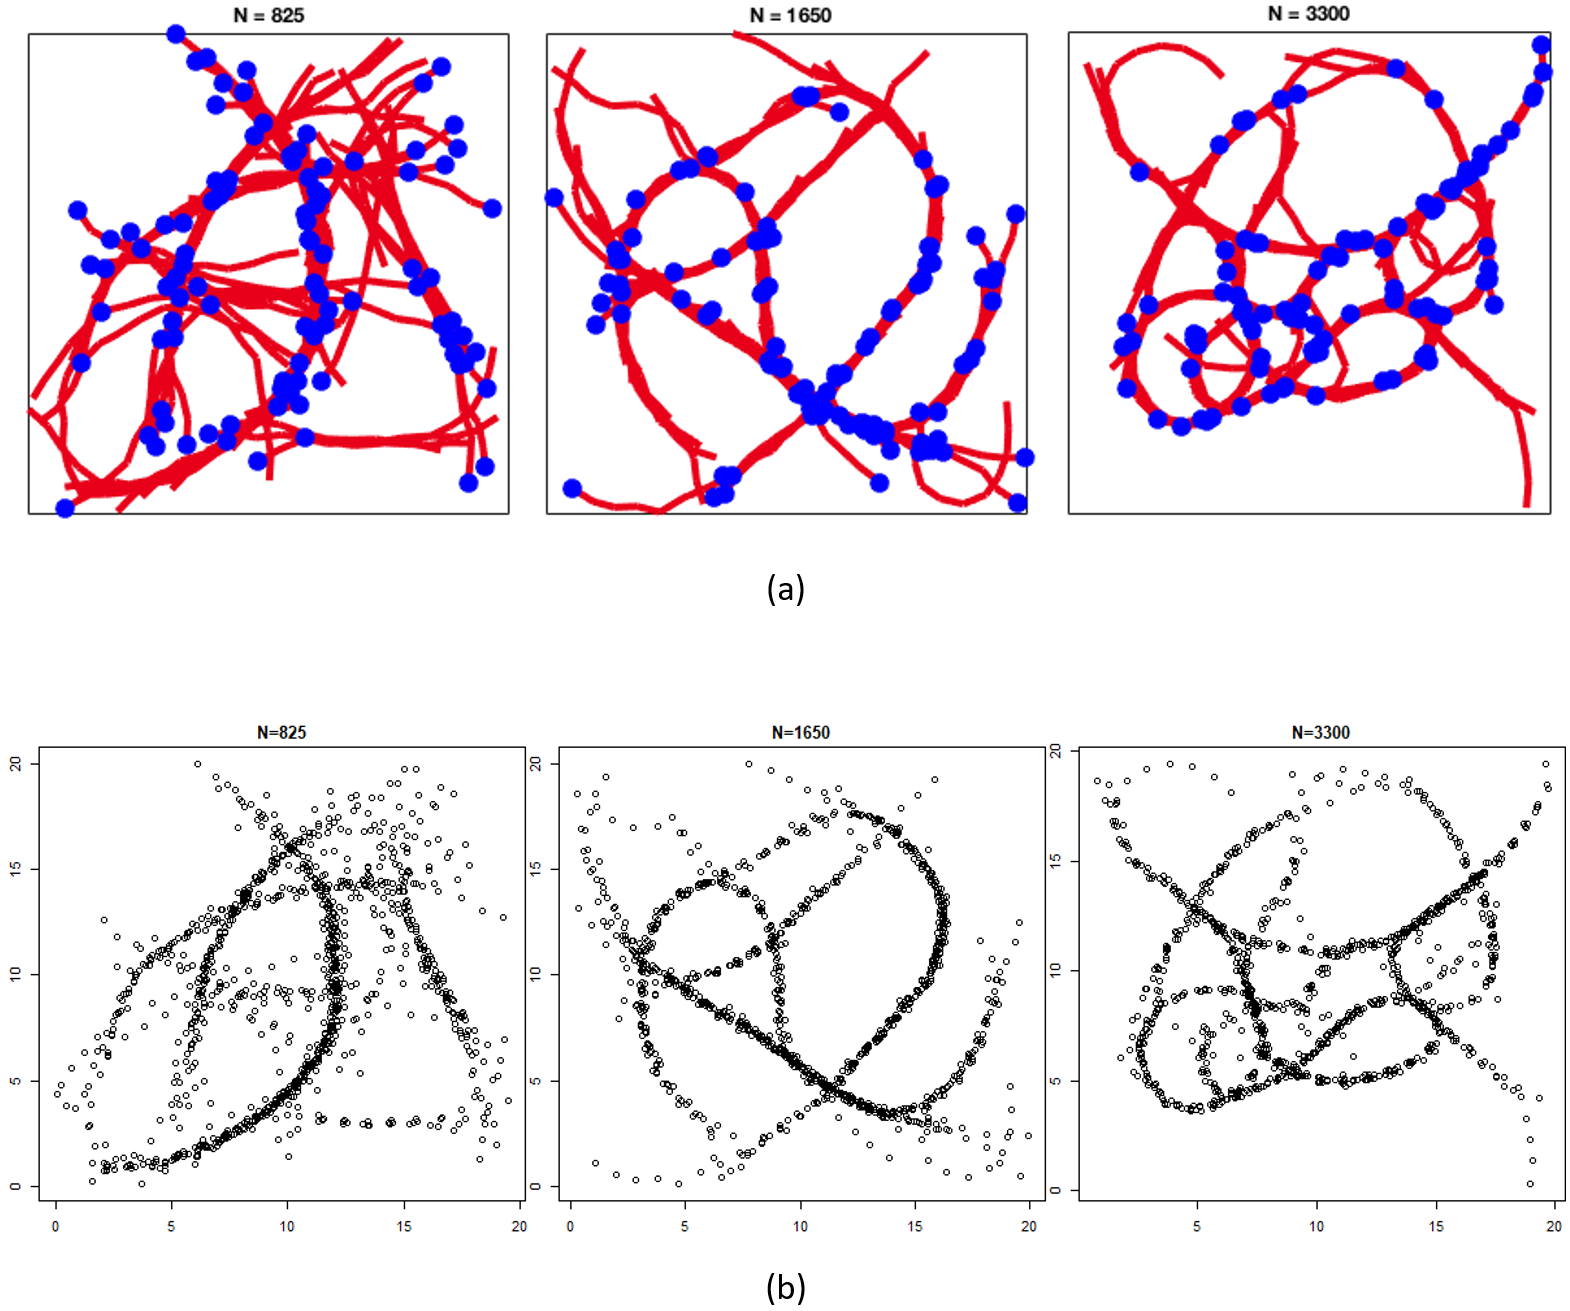
\includegraphics[width=1\textwidth]{rawdata.png}
	\end{center}
	\caption{Filament networks. Panel (a) shows three filament networks generated by $825$, $1650$ and $3300$ cross-linkers, respectively, in a $\SI{20}{\micro\metre} \times \SI{20}{\micro\metre}$ area. Each network contains $100$ filaments which are represented as red lines. The blue dots are the barbed ends of these filaments. Panel (b) shows the locations of the actin beads that make up the filaments exhibited in Panel (a).}
	\label{fig:rawdata}
\end{figure}

\subsection{Persistence Homology}
In order to build simplicial complexes, we adopt the procedure of forming Vietoris-Rips complexes on each dataset (actin network) by introducing a sequence of $\epsilon$-balls with increasing radius $\epsilon$ centered at each data point (a sampled pixel for image data or an actin bead in the synthetic data). Simplicial complexes are constructed based on intersections of these $\epsilon$-balls and each value of $\epsilon$ corresponds to an unordered group of homological features, which is called a homology group. Considering values of $\epsilon$ as a timeline, we only record when a homological feature appears and disappears. These indexes are called the birth times and death times of a particular homological feature. Moreover, the lifespan (death minus birth) of a homological feature is referred to as the feature's persistence. A set of homological features gives rise to a set of persistence measures. At the end of this procedure, when radius $\epsilon$ is sufficiently large so that the homology group remains unchanged by any further increase to the radius, information of a filament network's persistence homology (the set of persistpent homology measurements) is summarized in a persistence diagram.

\begin{figure}[!htbp]
	\begin{center}
		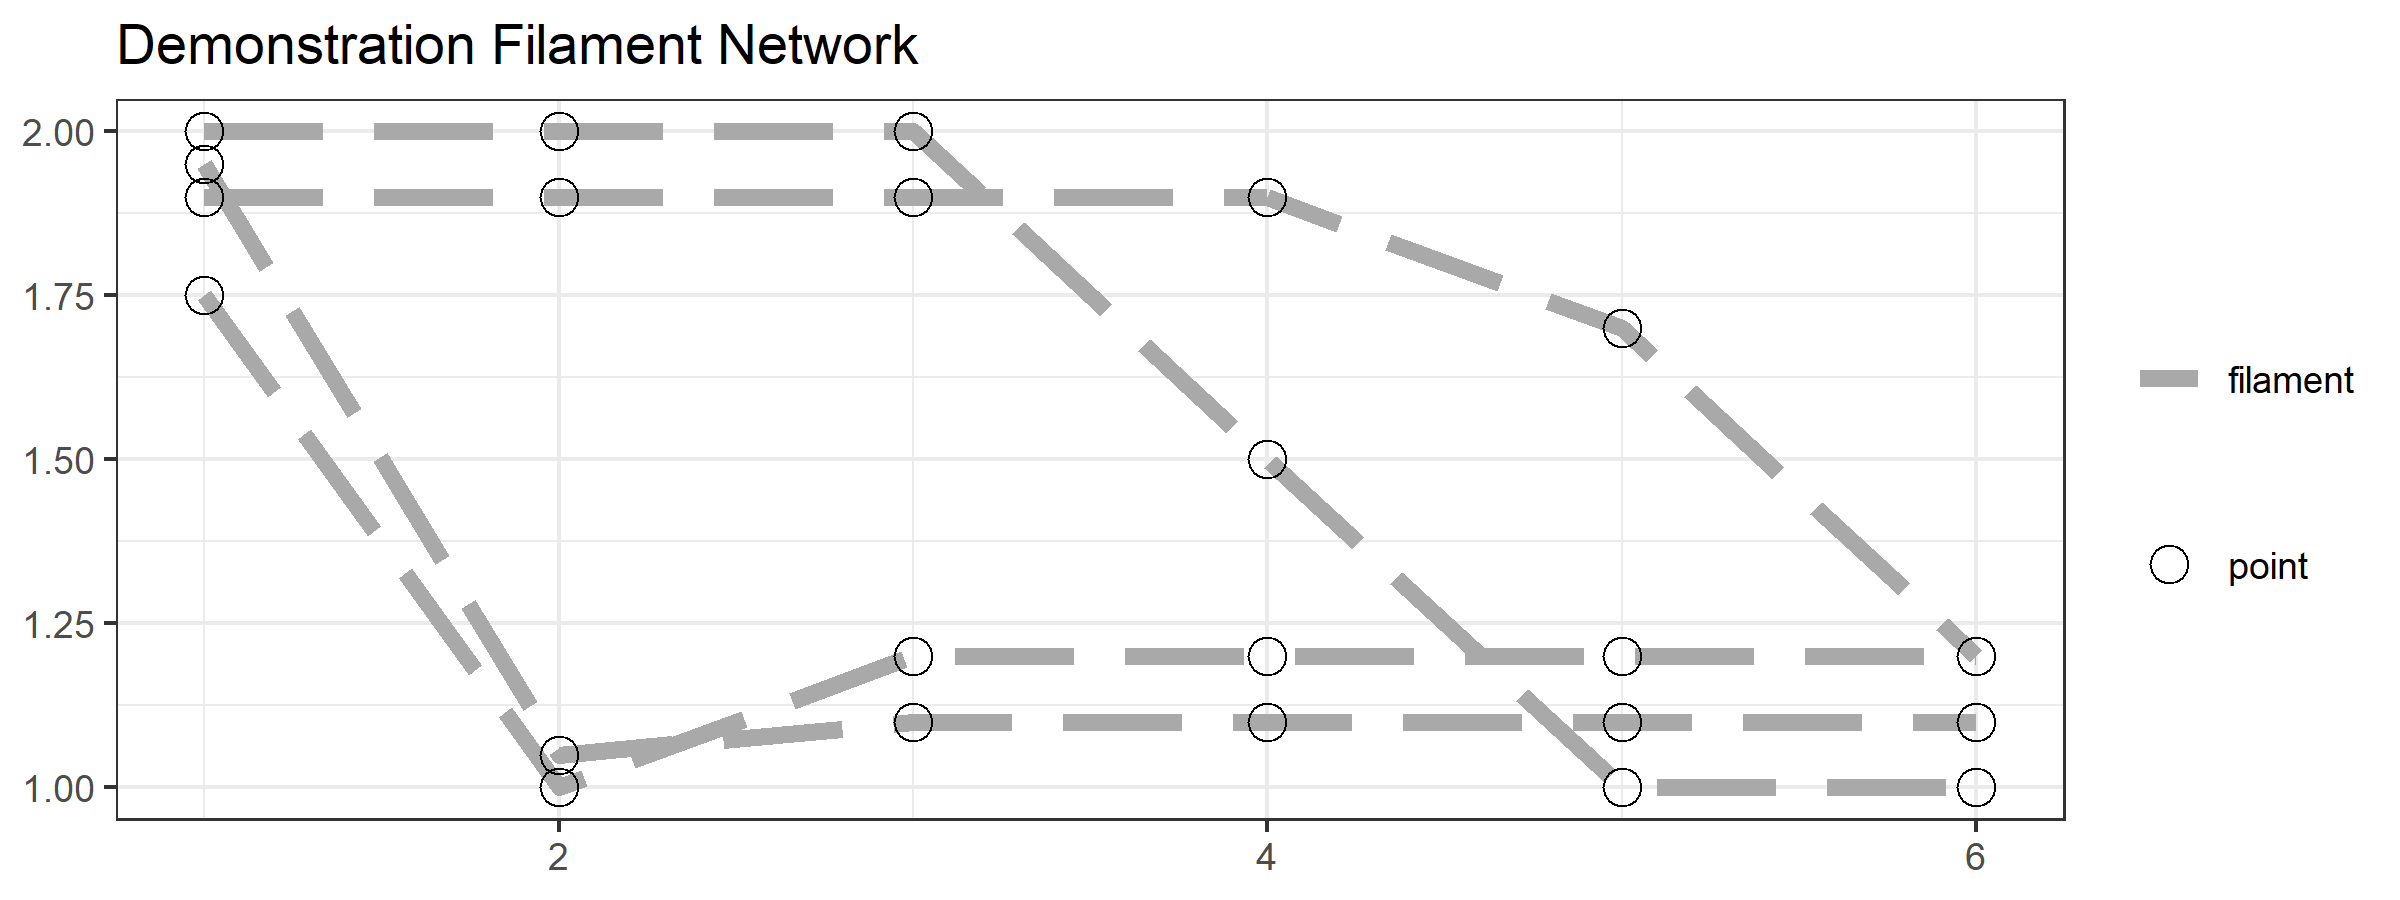
\includegraphics[width=1\textwidth]{figures/filaments_demo.png}
	\end{center}
	\caption{Demonstration fillament network. This network contains 3 filaments. Points are sampled along the filaments, in order to produce a point cloud from which persistence homology can be studied.}
	\label{fig:demoNetwork}
\end{figure}

For clarity, we demonstrate the formation of the persistence on a filament network. We use a simplified filament network which is shown in detail in Figure \ref{fig:demoNetwork}. Figure \ref{fig:persistencediagram} depicts the process of discovering and summarizing the persistence homology of the simple network shown in Figure \ref{fig:demoNetwork}. These illustrations should make clear the connection between filament networks, the Vietoris-Rips Complex and the encoding of the persistence information. 

\begin{figure}[!htbp]
	\begin{center}
		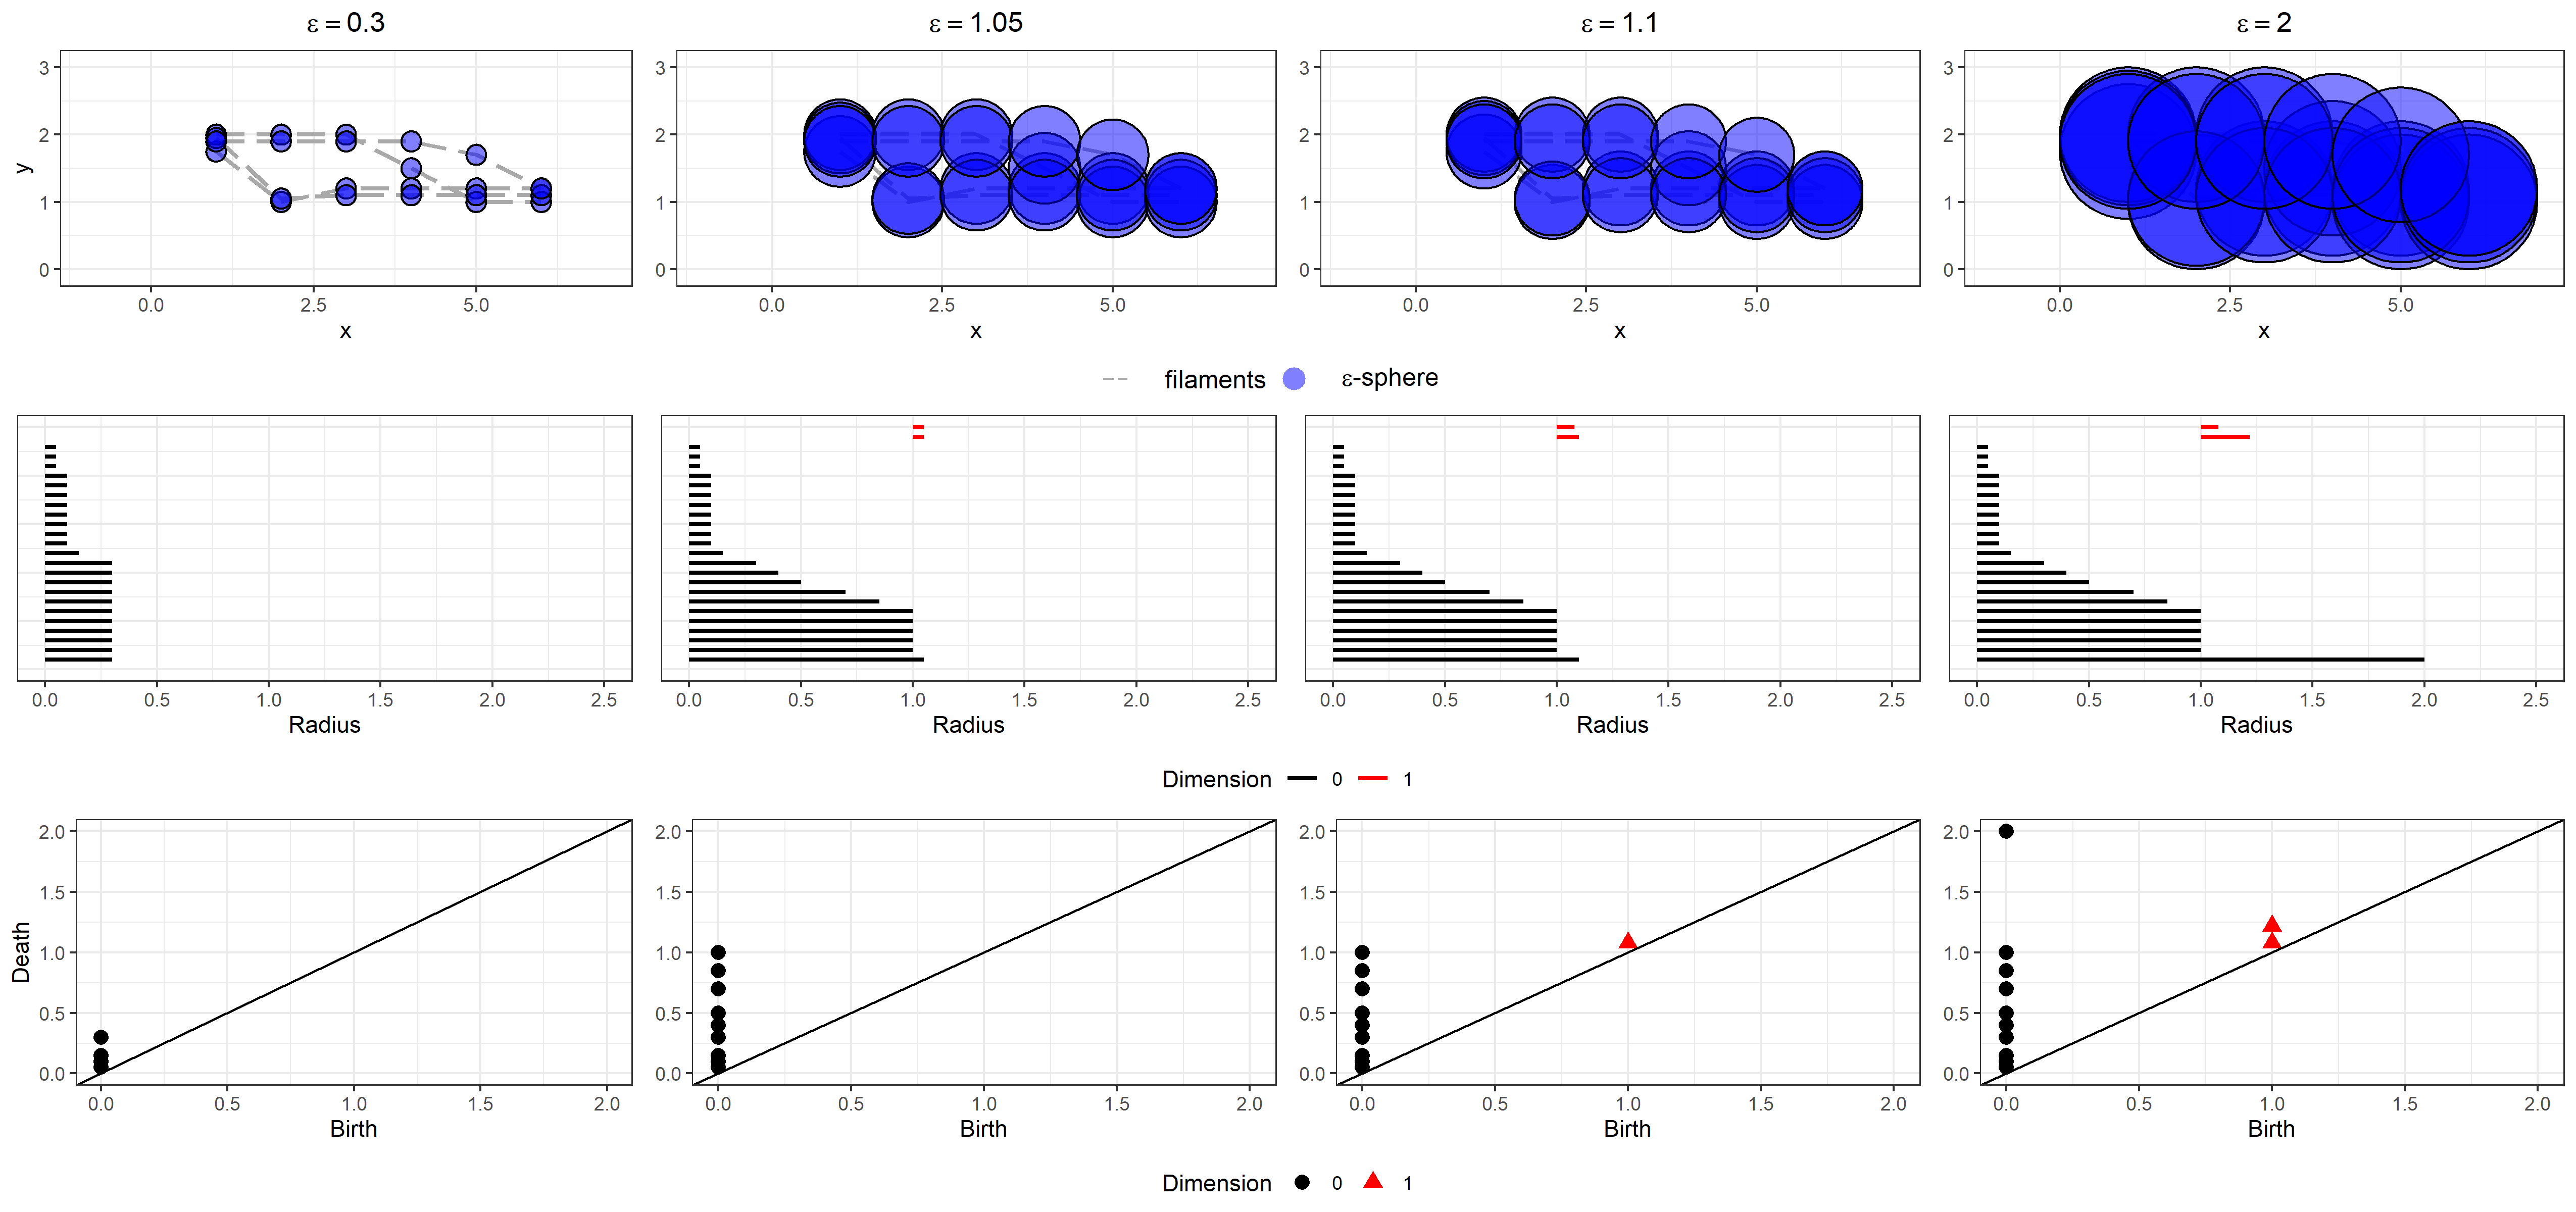
\includegraphics[width=1\textwidth]{figures/filaments_rips.png}
	\end{center}
	\caption{Investigation of the persistence homology of the demonstration filament network in Figure \ref{fig:demoNetwork}. The first row of figures, showes the growing $\epsilon$-spheres about the sampled points of the fillaments. The second row shows the corresponding persistence barcode. The third row shows the corresponding persistence diagram. The columns progress with the algorithm, right-to-left.}
	\label{fig:persistencediagram}
\end{figure}

When $\epsilon=0$, the sampled points of the filament network are each their own connected component. As the $\epsilon$-spheres grow, connecetd components begin to merge. In the first column of Figure \ref{fig:persistencediagram}, when $\epsilon=0.3$, several of the sampled points have already connected. We denote the points which have died (having connected into a larger connected component), by ending their bar in the persistence barcode below. In the third row (of persistence diagrams), we plot a point at 0 on the x-axis and at their precise time of death on the y-axis. When $\epsilon\approx1$, two holes form. The holes are evident in the top row, second column, of Figure \ref{fig:persistencediagram}, where one can see a larger and a smaller hole. We begin plotting bars for the holes in the corresponding persistence barcode below. Note that there are not yet reccords (points) for the holes in the persistence diagram. This is because we must know the death time of the holes in order to plot them in the 2-dimensional persistence diagram. 

In the third column of Figure \ref{fig:persistencediagram}, when $\epsilon=1.1$, the smaller hole has closed, and become part of a larger connected component. Now a single point is plotted in the persistence diagram below and the corresponding bar in the persistence barcode is terminated.

As the algorithm progresses, the larger hole eventually dies and its corresponding bar in the final persistence barcode is terminated. A point is also added at the corresponding birth and death in the persistence diagram (a second red triangle appears in the final column, bottom row of Figure \ref{fig:persistencediagram}). The algorithm could continue to $\epsilon=\inf$, but it is evident in this example that no more homologic information will be discovered as the spheres continue to grow. We choose to terminate the algorithm at $\epsilon=2$, terminate the final bar in the persistence barcode, and plot a point at (0,2) in the persistence diagram to denote final death time of the connected component which includes all the merged spheres.

Persistence homology indirectly summarizes the hidden shape of the data. In this work, we transcribe the persistence information of each cell to a persistence diagram. Having reccorded the persistence information of the networks, a classifier can be generated either from the distance \cite{marchese2018signal} between persistence diagrams or by alternative vectorizations of the diagrams \cite{adams2017persistence,bubenik2015statistical,maroulas2018stable}. Equipped with persistence diagrams, we will now detail several methods of classification built on the diagrams' homological information.












\clearpage	
%\nocite{*}
\bibliographystyle{plain}
\bibliography{bibliography}


\end{document}
